\subsection{\donutfull}
\label{subsec:donut}

\donut{} adalah sebuah transformer yang tidak memerlukan penggunaan \ocr{} untuk melakukan pemahaman terhadap dokumen. Konsep utama \donut{} adalah pemetaan langsung dari gambar dokumen mentah menjadi hasil yang terstruktur dan melewati seluruh proses implementasi \ocr \parencite{kim2021donut}. \donut{} merupakan sebuah \emph{pre-trained model} yang menggunakan \emph{visual encoder Transformer}, yaitu \swin{} untuk melakukan ekstraksi fitur visual dari dokumen, dan \emph{text decoder Transformer}, yaitu \bartfull. Oleh karena itu, \donut{} tidak memiliki ketergantungan pada fungsionalitas \ocr{} sama sekali.

\textit{Pipeline} implementasi \transformer untuk pemahaman dokumen pada umumnya terlihat pada \autoref{fig:non-donut-pipeline}. \donut{} menyederhanakan pipeline ekstraksi data dokumen seperti terlihat pada \autoref{fig:donut-pipeline}. Dengan implementasi \textit{pipeline} yang lebih sederhana, proses ekstraksi data dokumen dapat diproses secara \ee{} melalui Donut tanpa perlu melewati fase \textit{pre-processing} dan \textit{post-processing} dari gambar \textit{input} dan \textit{output}.

\textit{Input} gambar akan diterima oleh \encoder, seperti \swin{} atau ResNet yang akan memecah gambar menjadi gambar-gambar kecil yang tidak saling bertumpuk. Hasil dari \encoder{} akan dikirimkan ke \decoder{} \transformer{} yang digunakan, seperti BART, untuk diproses menjadi \textit{output} berbentuk deretan teks. \textit{Output} yang dihasilkan akan dikonversi menjadi format \jsonfull.

\begin{figure}[htbp]
    \centering
    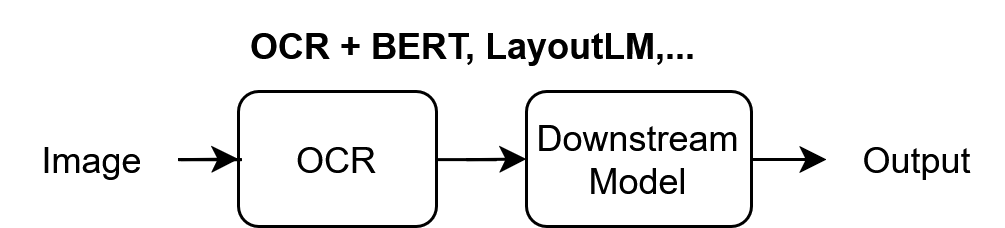
\includegraphics[width=0.8\textwidth]{images/non-donut-pipeline}
    \caption{\textit{Pipeline} sebelum implementasi \donut{} \parencite{kim2021donut}.}
    \label{fig:non-donut-pipeline} 
\end{figure}

\begin{figure}[htbp]
    \centering
    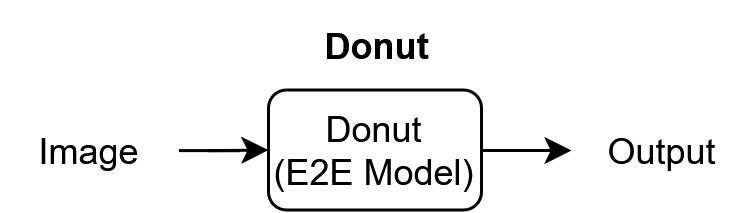
\includegraphics[width=0.8\textwidth]{images/donut-pipeline.png}
    \caption{\textit{Pipeline} setelah implementasi \donut{} \parencite{kim2021donut}.}
    \label{fig:donut-pipeline}
\end{figure}